\documentclass[12pt,a4paper]{journal}
\usepackage[margin=1in]{geometry}

\usepackage{times}

\usepackage[utf8]{inputenc}
\usepackage[T1]{fontenc}
\usepackage{indentfirst}
\usepackage{amsmath}
\usepackage{amsfonts}
\usepackage{amssymb}
\usepackage{caption}
\usepackage{subcaption}
\usepackage{graphicx}
\usepackage{siunitx}
\sisetup{range-phrase=--, range-units=single}

\graphicspath{{img/}}
\usepackage[numbers, super, sort&compress]{natbib}


\usepackage{tcolorbox}

\begin{document}

\section*{Retinal haemodynamics, vascular diseases, neovascular age-related macular degeneration and diabetic retinopathy}

\subsection*{Retinal haemodynamics}

\begin{figure}[t]
  \centering
  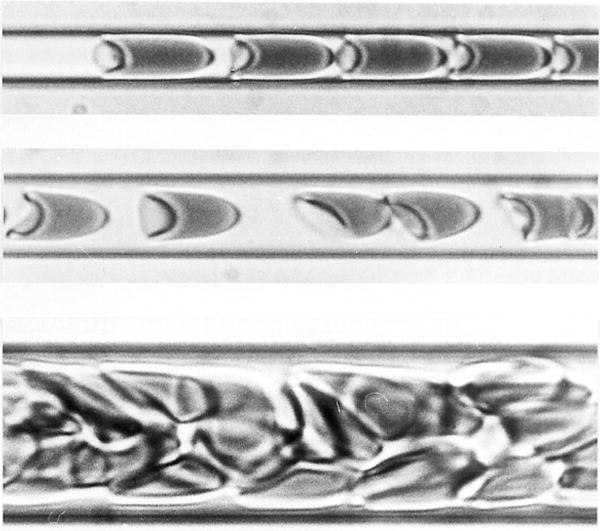
\includegraphics[width=0.45\textwidth, height=5.3cm]{cropped-RBC-in-capillaries.jpg}
  \hfill
  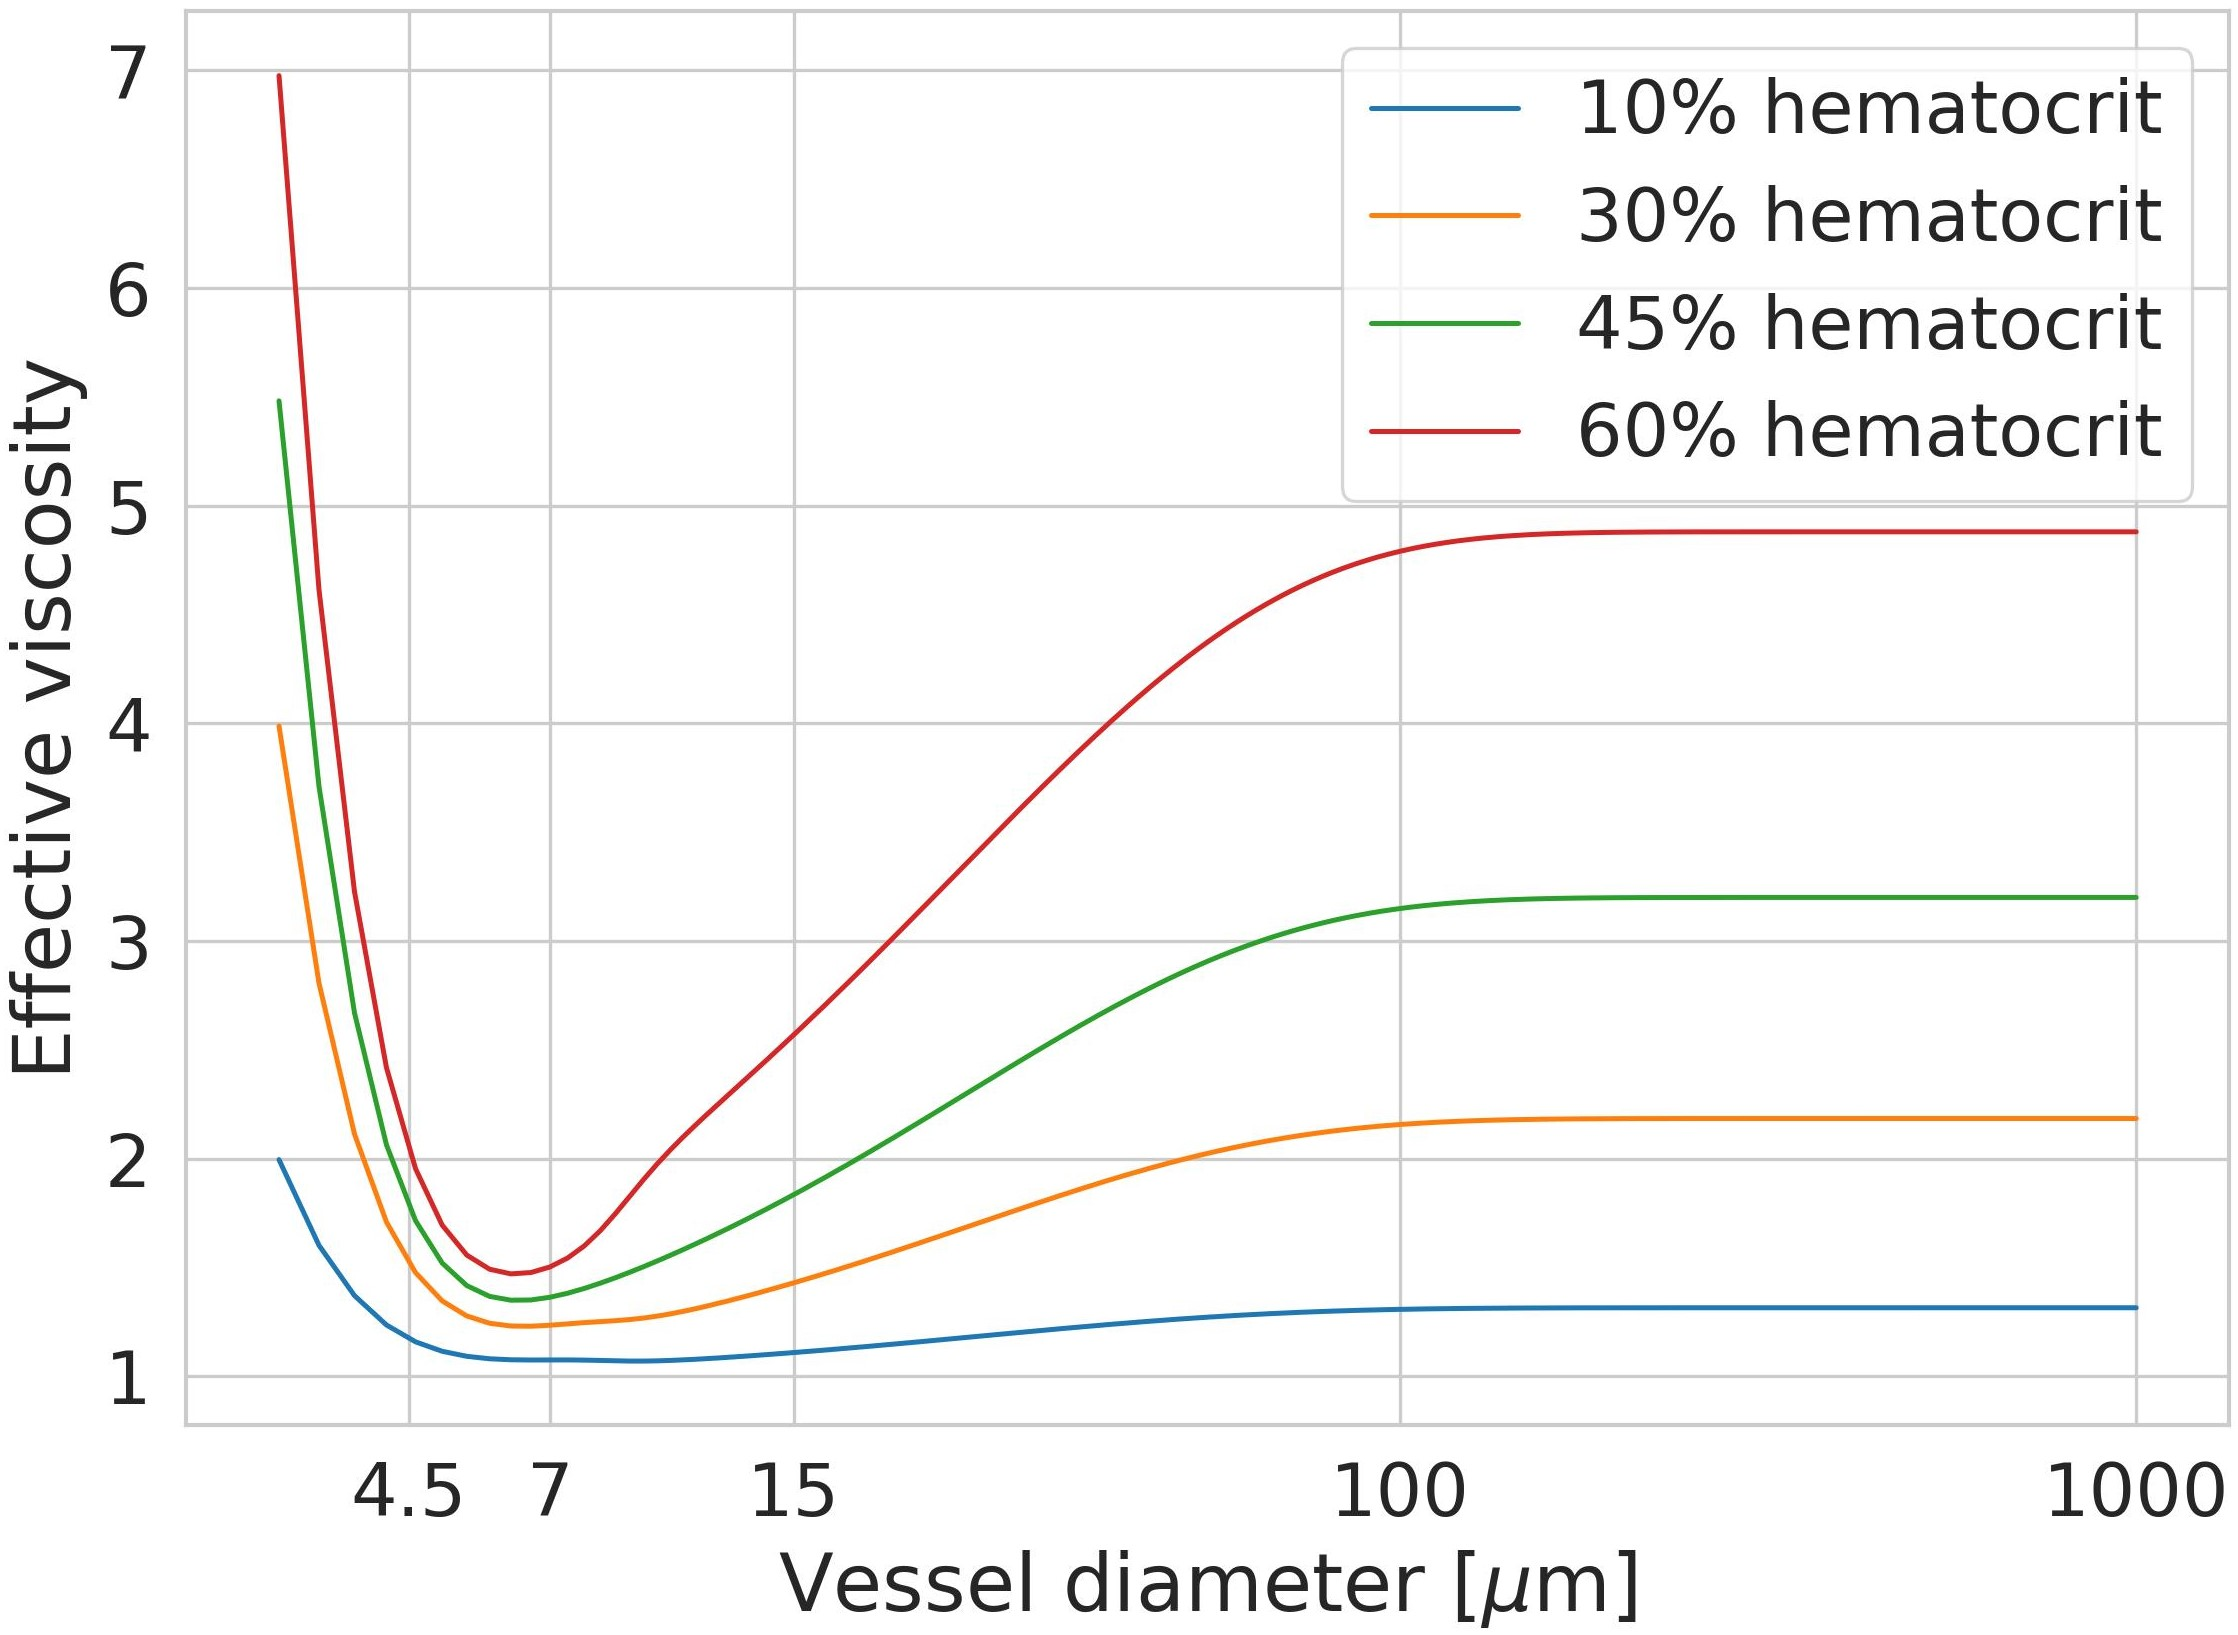
\includegraphics[width=0.45\textwidth, height=5.3cm]{EffectiveViscosity-Secomb.jpeg}
  \caption{Example of the effect of capillary calibre on the flow of blood. \textbf{Left}: Red blood cells in suspension in blood flowing within tubes of different diameter: \SI{4.5}{\micro\meter} (top), \SI{7}{\micro\meter} (middle) and \SI{15}{\micro\meter} (bottom). One can observe the flow of cells converging into a single file, surrounded by a layer of plasma as the diameter moves from \SI{15}{\micro\meter} to \SI{7}{\micro\meter}. The cell's shape adapt to fit into the tube as the diameter reaches the cell's size (top row). Reproduced with permission from Secomb.~\cite{Secomb_2003} \textbf{Right}: Example of an empirical law for the effective viscosity of blood accounting for the F\r{a}hr\ae us-Lindqvist effect and increased vascular resistance in smaller capillaries from the work of Secomb and Pries~\cite{Secomb_2013}.}
  \label{fig:effectiveViscosity}
\end{figure}

Adequate blood flow is essential for the supply of nutrients and removal of cellular wastes required to maintain visual functions.
The atypical dual circulation of the retina is both complex and fragile.
It is thought that the inner vessels perfuse the inner \SIrange{60}{80}{\percent} of the retina while the choroid supplies the remaining, more metabolically active, outer layers, around the photoreceptors.~\cite{Birol_2007}
It is also known that ocular blood flow is affected by, among other things, intraocular pressure, systemic blood pressure, metabolic activity and oxygen saturation of the blood.~\cite{Birol_2007,McCullough_1997,Palkovits_2014,Polska_2007,Pournaras_2008,Riva_1997,Wang_2014}
Many retinal disease have been linked, whether directly or indirectly, with abnormal haemodynamics.~\cite{Hayreh_2004,Medina_2016}

Retinal haemodynamics models are concerned with describing blood flow within the inner retinal or choroidal circulations and often rely on the Hagen-Poiseuille equation to determine flow in vascular segments.
This equation is a simplification of the more comprehensive Navier-Stokes equations made by making a number of assumption (see \textit{Additional information}).
The Hagen-Poiseuille equation states that blood flow ($Q$) in a vessel of length $L$ and radius $r$ is driven by a pressure drop ($\Delta p$) according to:
\begin{equation*}
  \label{eq:Hagen-Poiseuille}
  Q = \mathcal R\times\Delta p \mbox{, where } \mathcal{R} = \frac{8\mu L}{\pi r^4},
\end{equation*}
where $\mu$ is the apparent viscosity of blood which may account for changes in vascular resistance ($\mathcal R$) in vessels of varying diameter (see \textit{Additional information} and Figure~\ref{fig:effectiveViscosity}).
The fourth power of the radius in the formulation of vascular resistance describe the strong effect that even small contractions or dilations of a vessel can have on blood flow.
This relation between radius and flow is at the source of the autoregulation ability of blood vessels, which adapt their radius in response to a number of different cues.~\cite{Kur_2012}
The cellular constitution of retinal vessels suggests that blood flow is mainly regulated by arteries and arterioles.~\cite{An_2020,Kur_2012}
Evidence suggests that the choroid is also able, maybe to a lesser degree, to regulate blood.~\cite{Polska_2007,Riva_1997}
Neurological regulation (regulation by the autonomic nervous system) of choroidal blood flow has been suggested, in view of the rich innervation of choroidal vessels.~\cite{BeharCohen_2020,Polska_2007}

\textit{In silico} models provide valuable insights into the mechanisms that combine to provide healthy perfusion or, conversely, create conditions for the onset of retinal pathologies.
The assumptions made in these models can be validated by comparing simulation results and \textit{in vivo} measurements of changes of blood flow or vessel radii.
Vessel radius in the inner retina can be measured from retinal scans such as fundus photographs, fluorescein angiograms or optical coherence tomography (OCT) angiograms.
Blood flow can be measured using devices such as Doppler flowmeter or Doppler Fourier-domain OCT, in combination with radius measurements.~\cite{DoblhoffDier_2014,Wang_2009}
The blood's saturation in oxygen can also be measured \textit{in vivo}.~\cite{Geirsdottir_2013}
Reliable measurement of blood flow or vessel radii in the choroid is more difficult, though changes in haemodynamics can be observed \textit{in vivo}.~\cite{Riva_1997,Scherm_2019}

In this section, we review \textit{in silico} models that describe the normal physiology of the retina and models aiming at understanding the aetiology of various diseases which may be linked with haemodynamics in the retina and the underlying choroid.
More comprehensive reviews of models of the microcirculation, angiogenesis and oxygen delivery can be found in the work of Arciero et al.~\cite{Arciero_2017, Arciero_2019}

\begin{tcolorbox}[title=Additional information -- Fluid flow modelling]
  \begin{itemize}
  \item Viscous fluids such as blood are modelled by a set of differential equations relating acceleration, velocity, convection, density and pressure of a fluid called the Navier-Stokes equations.
    Solving those equations can be problematic in complex geometries, for example in a large network of vessels.
  \item Those equations simplify to the Hagen-Poiseuille equation (see main text) when assuming that the fluid is Newtonian and the flow incompressible and laminar.
    The equation Hagen-Poiseuille equation is relatively simple to solve, even on large vascular networks.
  \item An incompressible flow has a constant density regardless of the pressure and the fluid's properties are the same in all directions, namely, it is an isotropic fluid.
  \item A Newtonian fluid is a fluid which has a constant viscosity for given pressure and temperature, regardless of the amount of shear it is subject to.
  \item A Newtonian fluid flowing within a pipe is called laminar when fluid particles (e.g., red blood cells, blood plasma) move along smooth path with no mixing between each path.
    This kind of flow is opposed to turbulent flow, which appears when the velocity of the flow goes over a threshold determined by a combination of the fluid's viscosity and density and the pipe's dimensions.
  \item The propensity of a fluid to flow in either fashion is summarised by the dimensionless Reynolds number.
  \item Laminar flows show a parabolic velocity profile across the pipe, or vessel, cross section, with peak velocity at the centre and null velocity at the walls.
  \item As demonstrated by F\r ahraeus and Lindqvist, viscosity decreases with vessel width as red blood cells align into a single file, as illustrated in Figure~\ref{fig:effectiveViscosity}.~\cite{Faahraeus_1931}
  \item Empirical viscosity laws are used to account for the so-called F\r ahraeus-Lindqvist effect and the dramatic increase in vascular resistance seen in capillaries smaller than red blood cells, an example of which is shown in Figure~\ref{fig:effectiveViscosity}.~\cite{Haynes_1960,Pries_1990,Secomb_2013}
  \end{itemize}
\end{tcolorbox}


\subsubsection*{In health}

% \begin{itemize}
% % \item Measurement of blood flow: DoblhoffDier 2014 (Fourrier-domain Doppler OCT)
% % \item Measurement of oxygen in vessels: Geirsdottir 2013 (oxymeter: two fundus images with different wavelength, one sensitive to saturation)
% % \item Mathematical models of retinal blood flow are useful to understand the physiology of the retina and how it is affected by changes within or outside the retina
% % \item Baseline retinal haemodynamics by Takahashi
% % \item Arciero 2017 for review on microcirculation modelling
% % \item Gravity: Nelson, Salerni, Petersen
% % \item Heart rate/haemodynamics of the ONH: Jin 2020 More comprehensive FEM of ONH and influence of heart rate (stiffening of LC with higher HR, reduced pulsatility of blood)
% % \item Zouache on CC flow
% % \item Chivarali 2021 on in series/parallel organization of the capillaries
% % \item Bernabeu 2014 on haemodynamic in the developing retina + Paul's review?
% % \item Looking into oxygen: Aquah, Causin 2016, Liu 2009
% % \item Autoregulation: Arciero 2008 (impaired regulation at low perfusion pressures, e.g., increased IOP; metabolic or carbon dioxide mechanisms are essential to autoregulation, impairement of both lead to a decrease of 95\% in autoregulation capacity), Arciero 2013 (supports that arteriole's contraction is regulated by saturation levels in the venules/capillaries by release of ATP from RBC), Guidoboni 2014a, Aschinger 2017 tested several 
% % \item Realistic vascular geometries: Liu 2009, Malek 2015, Rehban 2019
% \end{itemize}

The current understanding of the perfusion of the retina is still lacking.
A significant effort has been made in modelling the complex circulatory systems that perfuse the retina in order to complete it.


Takahashi et al. proposed an arterio-venous dichotomously branching and symmetric network where all vessels within a given generation are identical.~\cite{Takahashi_2009}
The diameter and length of the branching vessels follows the principle of least energy described by Murray's law.~\cite{Murray_1926}
This theoretical model was used to describe the distribution of flow and other haemodynamic parameters across the normal retinal vasculature.
While clinical studies often report changes in the diameter of large retinal vessels in various conditions, its relationship with total retinal blood flow, a clinically relevant parameter, is unclear.
The network by Takahashi et al. has been adapted to further investigate the physiology of the retinal vessels, in conjunction with clinical experiments.~\cite{Aschinger_2017,Pappelis_2020}
One of those studies showed that changes in total retinal blood flow is not linearly related with dilation of larger vessels but that, in fact, the diameter of the capillaries has the strongest impact on vascular resistance.
The patterns of vasodilation tested, however, assumed that the capillaries are able to vary their diameter when the validity of such assumption is still unclear.~\cite{Kur_2012}

The other study used clinical information to create patient specific networks based on the method of Takahashi et al.~\cite{Pappelis_2020}
The model included a autoregulation component as a function of retinal perfusion pressure (pressure entering the central retinal artery, estimated as a difference between systemic blood pressure and intraocular pressure), and predicted the blood flow response to increases in intraocular pressure or drops in retinal perfusion pressure.
This allowed prediction of the autoregulation capacities of retinas in patients treated for hypertension or in eyes subject to ocular hypertension.
It showed that the retinas of both healthy and hypertensive patients was closer to the lower limit of autoregulation, suggesting that the retina may be more sensitive to decreases rather than increases in perfusion.~\cite{Pappelis_2020}


Lumped parameters models have been used to investigate the relationships between intra- and extra-vascular pressures and haemodynamics in the retina and choroid.~\cite{Chiaravalli_2021,Fawzi_2019,Guidoboni_2014a,Nelson_2017,Petersen_2022,Prudhomme_2021,Sala_2020,Salerni_2019}
In those models, similar vessels are sorted into compartments, e.g., central retinal artery, arterioles, capillaries, venules, central retinal vein and choroid.
The physical processes within compartments and the interactions between them are summarized by few parameters.
In analogy with electrical circuits, haemodynamics in each compartment is characterised by a resistance, the combined effect of the vascular resistance of a compartment's vessels, and a capacitance, the total amount of blood that can be stored in the same vessels.
Autoregulation mechanisms impact the capacitance of a compartment, while pressures affect the resistance coefficient.

Lumped paramteres models have been used to investigate the links between gravity-induced shifts in intracranial fluids, ocular fluids and pressures and the loss of sight observed in astronauts.~\cite{Nelson_2017,Petersen_2022,Salerni_2019}
Nelson et al. proposed a baseline model simulating increases in ocular pressures secondary to such fluid shifts.~\cite{Nelson_2017}
The simplistic model predicted relatively well the response of intraocular pressure to changes in the gravitational environment or tilt of the body.~\cite{Nelson_2017,Petersen_2022}
A more comprehensive model including interacting brain, body and eye compartments showed that the retinal circulation was relatively spared from hypoperfusion compared to the choroidal circulation in microgravity conditions.~\cite{Salerni_2019}

Several lumped parameters models have been developed to better understand the mechanisms behind autoregulation in physiological conditions.~\cite{Arciero_2008,Arciero_2013,Guidoboni_2014a}
Arciero et al. used a symmetric network similar to the one by Takahashi et al. to understand the information pathways leading to blood flow autoregulation in the retina.~\cite{Arciero_2008,Arciero_2013}
Both models assumed that only arterioles possessed the ability to contract to regulate flow.
These models were used to investigate the response of individual or combined autoregulation pathways to changes in perfusion pressure or oxygen consumption rate of the cells.
The earliest model investigated the hypothesis that arterioles can contract in response to the oxygen saturation of blood in the downstream venules.~\cite{Arciero_2008}
The study showed that such autoregulatory pathway could account for the experimentally observed response of perfusion to changes in consumption rates.
This mechanism, along with other known ones, have been modelled together in a subsequent study.~\cite{Arciero_2013}
In this study, the contributions of each pathway to retinal perfusion was assessed.
The results showed that the arterioles' responses to carbon dioxide concentration in the surrounding tissue and oxygen saturation in the venules were essential to retinal autoregulation.~\cite{Arciero_2013}

Guidoboni et al. looked at the interplay between intraocular pressure, retinal haemodynamics, systemic blood pressure and autoregulation.~\cite{Guidoboni_2014a}
Instead of the mechanistic description of autoregulation proposed in the work by Arciero et al., they used an empirical response function of arteriole diameter to changes in perfusion pressure.
Another difference with the previous work is the assumed capacity of the venules and central retinal vessels to dilate or collapse, passively and to some limited extent, in response to pressure gradients across their walls.
The retinal haemodynamics of six types of physiology (high, normal or low blood pressure, with or without working retinal autoregulation) were simulated across a range of intraocular pressure.
The model predicts the ranges of intraocular pressure within which each physiology can maintain relatively constant blood flow.
The dependence of these ranges to systemic blood pressure and autoregulation capacity may explain some discrepancies regarding the effects of intraocular pressure on retinal haemodynamics found in experimental studies.~\cite{Guidoboni_2014a} 

The transport and delivery of oxygen to the tissue has been modelled by several groups.~\cite{Aquah_2021,Causin_2015,Liu_2009}
The earliest one used a short arteriolar tree, taken from a retinal photograph of a healthy young volunteer, and solved the Navier-Stokes equation to obtain haemodynamics of blood in these vessels.~\cite{Liu_2009}
The downstream vasculature was represented as a structured tree extending the outlets of the segmented arterioles.
This model reproduced the distribution of intravascular oxygen observed \textit{in vivo} and could serve as a baseline to analyse oxygen distribution in realistic vascular networks.
However, reproduction of the retinal vasculature is limited to larger vessels.
Therefore, the use of artificial vasculature with similar characteristic as the real one may be useful to model the whole extent of the retinal vasculature.

Causin et al. used the fractal similarity between retinal vessels and diffusion-limited aggregation process to generate a three dimensional network of three of the vascular plexi of the retina.~\cite{Causin_2015}
Oxygen transport throughout the extensive vascular network was modelled as well as the oxygen delivery to the tissue, modelled as a rectangular slab.
The good agreement with data validated the use of the artificial networks.
The effects of haemodynamics parameters on different parts of the tissue and the vasculature was analysed with the model and showed, among other things, the sensitivity of perfusion of retinal ganglion cells to blood viscosity and metabolic consumption.~\cite{Causin_2015}


Several other studies have used vessels reproduced from images to analyse the distribution of blood flow and the influence of the morphology.~\cite{Malek_2014,Malek_2015,Rebhan_2019}
Malek et al. tried to characterise the flow distribution in reproduced arterioles and veins to quantify the impact of vessel tortuosity on haemodynamics parameters.~\cite{Malek_2014,Malek_2015}
The deformation of vessels caused by the pulse of blood is a computationally complex task to model and a simplified model has been developed and applied to a similar reproduction of the retinal vasculature, with a brief analysis of its effects on haemodynamics.~\cite{Aletti_2016}
Notably, Rebhan et al. have looked at the interactions of retinal haemodynamics and tissue stress using reproductions of the large vessels of healthy and diseased eyes, an aspect previously overlooked that may have importance in, e.g., glaucoma and diabetes.~\cite{Rebhan_2019}


Others have used finite element modelling, a technique suitable for modelling of mechanistic forces, to understand the blood flow in the central retinal vessels.~\cite{Guidoboni_2014,Jin_2020}
The central retinal vessels enter the retina along the optic nerve where they are under pressure from the surrounding tissue, the cerebrospinal fluid surrounding the eye, the intraocular pressure and, potentially, the artery and the vein may also compress each other.~\cite{Nickells_2012}
The lamina cribrosa's purpose is to act as a buffer protecting the vessel where all those pressures confront each other.
Guidoboni et al. simulated the displacement of the lamina cribrosa and the stress due to different intraocular pressures and pressure induced by the cerebrospinal fluid.~\cite{Guidoboni_2014}
The predictions of blood flow in the central retinal artery showed good agreement with measurements made during intraocular pressure elevation, suggesting that the observed decrease in blood flow velocity is caused by the lamina cribrosa compressing the artery.
Note that this model assumed a constant blood pressure, average of the systolic and diastolic blood pressures.
Pulsatility may have a significant impact on intraocular pressure and, consequently, blood flow in the central retinal vessels and has been investigated within a more comprehensive model of the ocular structures.~\cite{Jin_2020}


Whether the vascular plexi in the retina, namely, the superficial, intermediate and deep plexi, are connected \textit{in series} or \textit{in parallel} is still unclear.
The \textit{in parallel} configuration suppose that both arterial and venous connections exist between plexi.
Conversely, in the \textit{in series} configuration, blood inflow comes solely from the superficial plexus, while venous drainage happens only in the deep plexus.
We refer the reader to Figure 1 in the paper by Chiaravalli et al. for a schematic of those two configurations.\cite{Chiaravalli_2021}
The lumped parameter models developped in this paper simulate haemodynamics between the central retinal artery to the central retinal vein in five vascular compartments.~\cite{Chiaravalli_2021}
The authors modelled both configurations and compared the responses of each plexi to intraocular pressure elevation and occlusion of the central retinal vein.
The model showed that the \textit{in series} configuration better captured the response observed in clinical studies, and may better describe the actual physiology of the retinal vasculature.


\textit{In silico} models have also been developed to understand how the retinal vasculature develops.
A review of some of those models can be found in other reviews.~\cite{Arciero_2019,Roberts_2016}
However, the role haemodynamics plays in the angiogenesis of the vascular beds is still elusive.
Bernabeu et al. proposed a model of blood flow in a reconstructed murine vasculature that can be used to simulate the haemodynamics forces that cannot be measured in small capillaries but may affect angiogenesis.~\cite{Bernabeu_2014}
Others looked at how the branching patterns in the early development of the murine retina may affect later development.~\cite{Mirzapour_Shafiyi_2021}
The results showed that hyper-branching behaviours in the young vascular bed reduces the blood supply, and hence the oxygen, at the growing ends of the vasculature.
The lack of oxygen on this front may drive up-regulation of vascular growth factors promoting vascular growth.


The use of realistic vascular networks provides a link between haemodynamics and clinically relevant indices.
The effect of tortuosity of the vasculature has been investigated on short, segmented sections of the retinal veins.~\cite{Malek_2014}
In this model, the Navier-Stokes equations are used to find flow within the arterioles, while peripheral circulation is accounted for by an impedance condition at the outlets of the segmented tree.



While the inner retinal vasculature feeds the inner third of the retina, the remaining two thirds are perfused by the choroidal circulation.
In contact with the retina is the choriocapillaris (CC) layer of the choroid.
The CC provides oxygen across the Bruch's membrane to the photoreceptors and other neuronal cells of the outer retina through diffusion only.
Therefore, a high vascularisation is necessary to provide enough oxygen despite the distance.
Defects in choroidal blood flow are associated with major retinopathies such as nAMD and DR~\cite{Pemp_2008}.
Despite its importance, little is known about the physiology of the choroid.
Likewise, little work has been done on modelling choroidal circulation.
Early work tried to decipher whether the choroid of rabbits was able to regulate its flow in response to changes in systemic pressure.\cite{Kiel_1992}
Simulations in pair with experimental evidence suggests a autoregulatory reflex in the choroid triggered by blood pressure.
Since then, only Zouache et al. modelled the physiology of choroid and its peculiar architecture~\cite{Zouache_2015}.
By simulating the lobular structure of the CC, they investigated the effects of the geometry of lobules on the flow of blood.
Their work suggested that the distribution of flow separators in the CC and the location of inlet and outlets in individual lobules may explain the localisation of oedema or neovasculature in diseased eyes.\cite{Zouache_2015}



\subsubsection*{In disease}

Many retinal pathologies have or may have a link with irregular haemodynamics.

The model by Rebhan et al. previously discussed compared haemodynamics in vascular networks segmented from a healthy eye and eyes affected by glaucoma or diabetes.~\cite{Rebhan_2019}
The embedding of the vessel in the tissue revealed an increase in wall shear stress in the diseased eyes compared to the healthy one.
However, it was noted by the author that the absence of the downstream vasculature is likely to affect the quality of predictions.\cite{Rebhan_2019}
Along the same lines, higher vascular tortuosity, a common sign of ageing and disease, has been shown computationally to increase the pressure drop across the vasculature.~\cite{Malek_2014}
However, vessel-tissue interactions were not considered in the model.


Numerous models have been developed to explain alterations of blood flow observed in eyes subject to glaucoma or vessel occlusion.\cite{Chuangsuwanich_2016,Guidoboni_2014,Sala_2018,Sala_2020}
Elevated intraocular pressure, a hallmark of glaucoma, is expected to affect the retinal circulation, causing loss of sight.
Modelling of the interactions between the ocular structure surrounding the central retinal vessels has shown the role of a stiffened lamina cribrosa resulting from such conditions.~\cite{Guidoboni_2014}
In addition, the model showed that the geometry of the sclera and the lamina cribrosa affect the sensitivity of blood flow to elevation of intraocular pressure.
This framework was extended in Sala's thesis to create the Ocular Mathematical Virtual Simulator, a simulation environment for the interactions of haemodynamics and biomechanics in the eye.~\cite{Sala_2018,Sala_2020}
The environment allowed to simulate haemodynamics of individual patients characterised by a handful of parameters, yielding significantly different results for each combination of parameters.
Results showed that high intraocular pressure can cause collapse of the central retinal vein and major differences in the displacement of the lamina cribrosa.
Interestingly, it showed that the perfusion of the lamina cribrosa is also negatively affected by ocular hypertension, a potentially significant mechanism in the understanding of glaucoma.~\cite{Sala_2020}
Perfusion and haemodynamics within the lamina cribrosa has been modelled separately using a large number of artificial capillary networks statistically representative of different morphologies of the lamina cribrosa.~\cite{Chuangsuwanich_2016}
For a review of the use mathematical models in glaucoma research, we refer the reader to the review by Harris et al.~\cite{Harris_2013}


Microaneurysms are an early manifestation of diabetic retinopathy where the walls of capillaries form outpouchings disrupting blood flow and which are susceptible to rupture.
We found four studies investigating haemodynamics in reconstructed microaneurysms using computational fluid dynamics models.~\cite{Bernabeu_2018,Czaja_2022,Li_2020,Li_2022}
One looked at the shape of microaneurysms and how it influences haemodynamics, and in particular shear rates, in an attempt to determine predictors of the likelihood of leaking blood clotting.~\cite{Bernabeu_2018}
Similarly, Czaja et al. investigated wall shear stress in microaneurysms in the event of stiffened red blood cells, another symptom of diabetes.~\cite{Czaja_2022}
A notable difference with the previous model, however, is the use of cell resolved blood flow simulations, where individual cell are modelled and transported by blood flow.
This allowed to investigate separately the flow of red blood cells and platelets cells and showed the differences in penetration through the microaneurysm between the two cell types.
The stiffened red blood cells were found to induce higher wall shear stress, both in the aneurysm sac and in the vessels feeding and draining it.
In two studies, Li et al. have also simulated the flow of red blood cells and platelets in microaneurysms with a focus on the platelet flow through the microaneurysm, as they may be linked with the formation of blood clots.~\cite{Li_2020,Li_2022}


Eyes with visual impairments such as myopia progressively affect the shape of the retina and may develop neovasculature.~\cite{Medina_2016}
This suggests a link between the curvature of the eye and retinal perfusion.
However, the effects of curvature have been assumed insignificant in most haemodynamics models to date.
Dziubek et al. modelled this curvature by representing the retina as a thin, curved surface, within which an artificial network of vessels is embedded.~\cite{Dziubek_2015}
Interestingly, vessels are considered as pores in the tissue and, therefore, blood flow was modelled using Darcy's law, which describes flow through a porous medium.
Therefore, arteriolar, capillary and venular networks are kept virtually separated but communicate through a `hierarchical' velocity variable, as opposed to the spatial velocity which transports blood throughout the retinal surface.
The dichotomous tree proposed by Takahashi et al. was used to generate the networks.
The model confirms clinical suspicions of a change in retinal haemodynamics due to ocular curvature.
Furthermore it highlighted the non-uniform effects on the retina, with the temporal region being less affected by ocular shape.\cite{Dziubek_2015}


Panretinal photocoagulation therapy is a common procedure to treat the ischaemia in retinae with proliferative diabetic retinopathy.
While practice has shown the efficiency of the procedure, its mechanisms of action remain unclear.
It is thought that procedure treats retinal ischaemia by reducing the oxygen consumption of the photoreceptors affected by the laser-induced burn.~\cite{Fawzi_2019,Gast_2016}
However, effects of the therapy on blood flow has been observed.
With a simple lumped parameter model and the assumption that panretinal photocoagulation increases vascular resistance in the periphery of the macula, Fawzi et al. showed how the surgery could increase macular blood flow.~\cite{Fawzi_2019}
The increased perfusion in the macula would then explain the decrease in VEGF concentrations and the subsequent regression of neovasculature.
The models predictions are along the lines of the seemingly increased flow in macular capillaries.~\cite{Fawzi_2019} 
The patterns of burn used in panretinal photocoagulation is also subject to debate.
Gast et al. investigated the effects of different patterns on the propagation of ischaemia due to capillary occlusion.~\cite{Gast_2016}
The model showed how different patterns of burn affect the propagation of ischaemia and suggest that targeting the non-ischaemic peripheral retina with appropriate patterns may be effective at containing it.


% \begin{itemize}
% \item Microaneurysm: Bernabeu 2018, Li 2020, Li 2022, Czaja 2022 
% \item Study of structure on perfusion capability of the retina (Lamina cribrosa in glaucoma: Changsuwanich, retinal curvature in e.g. myopia: Dziubek)
% \item Diabetic retinopathy: Czaja 2022, Bernabeu 2018, Rebhan 2019 (wall shear stress in realistic vascular network and stress on tissue; Difference in WSS between diseased and baseline but not in tissue stress)
% \item Photocoagulation: Fawzi 2019 using the electrical circuit analogy showed that panretinal photocoagulation works thanks to an improve in blood flow in the macular capillaries driven by an increase in vascular resistance in the peripheral retinal circulation. The model's results are in accordance with the observations. Gast 2016, very simplified vasculature to test the impact of burn patterns on oxygen, VEGF realease and how ischaemia propagates; Flower et al (simplistic, theoretical, shows that targeting the veins of the CNV rather than the CNV itself may be as efficient)
% \item Modelling the optic nerve: Band, Spelman, previous version of the section
% \item Glaucoma, retinal vein occlusion: Sala thesis (haemodynamics and structure modelling and their interactions, collapse of CRV from high IOP, time depedent, platform to simulate virtual patient's eyes based on a handful of parameters, mostly pressures; Extended from Guidoboni to account for perfusion and mechanic stress in the lamina cribrosa and the sclera;), Guidoboni 2014 (observed decreased blood flow velocity during IOP elevation is caused by compression of the CRA by the lamina cribrosa, dimensions of sclera and lamina cribrosa impact the sensitivity of blood flow to IOP changes); Harris 2013 review of mathematical models of haemodynamics in glaucoma; Rebhan 2019 (wall shear stress in realistic vascular network and stress on tissue; Difference in WSS between diseased and baseline but not in tissue stress);  
% \end{itemize}







\subsection*{Anti-VEGF}

In proliferative DR and nAMD, loss of sight is linked to detachment of the retina and accumulation of fluids or oedema~\cite{Roberts_2020, Waldstein_2016}.
Those are consequences of the growth of leaky blood vessels, referred to as neovasculature, in the neuronal retina and, in particular, in the macula.
The angiogenesis of macular neovasculature (MNV) is driven by gradients of vascular endothelial growth factors (VEGF) which are upregulated by hypoxia (a lack of oxygen) in the diseased retina.
Binding of free VEGF molecules to their receptors on the walls of existing blood vessels triggers the migration of the endothelial cells constituting said vessel walls.

The treatment of MNV is predominantly done via frequent injections of VEGF-inhibiting molecules that bind to the free VEGF present in the retina, ultimately inhibiting the angiogenic process.
These injections are typically done directly in the vitreous humor of the eye with a needle, though alternative delivery techniques are being investigated~\cite{Kim_2021}.

Molecules present in the vitreous are naturally eliminated through the aqueous humour flow, referred to as the anterior clearance route.
The posterior clearance route refers to clearance through the choroidal circulation.
In addition, the inner limiting membrane (ILM) and retinal pigment epithelium (RPE), respectively on the inner and outer retina, act as barriers to the molecules~\cite{Park_2015}.
Therefore, the presence of the drug in the retina and the choroid is limited to a fraction of the injected dose. 

Despite its general efficacy, current treatment strategies are sub-optimal for some patients in terms of dosage and interval between injections.
Eyes showing little to no improvement to their condition are referred to as non-responsive and present a real challenge for clinicians.

Furthermore, VEGF induced angiogenesis is a natural response to inflammation and hypoxia, in the eye and the rest of the body. 
Therefore, repeated injections pose a number of problems.
Firstly, the intravitreal injections (IVI) can cause further inflammations within the retina, triggering additional VEGF upregulation~\cite{Iyer_2022}.
Secondly, with the current doses, the unbound anti-VEGF molecules that are cleared from the eye are found in significant levels in the systemic circulation, raising concerns about the safety of IVI.
Indeed, while it is still matter of debate, it has been suggested that IVI of anti-angiogenic molecules could be linked with serious adverse effects including haemorrhages and strokes~\cite{Avery_2016, Kaiser_2019, Maloney_2021}.

Knowledge of the determinant of the total exposure of the retina and the choriocapillaris to the drug is important to develop better therapeutics molecules and administration strategies and reduce risk and burden on the patient.

However, while aqueous and vitreous humors can be sampled \textit{in vivo}, the concentrations in the retina and choroid remain unknown. 
Therefore, estimates of the retinal kinetics of molecules are often based on either animal experiments or on samples of the aqueous humor, the vitreous humor and systemic plasma.
Mechanistic pharmacokinetic (PK) and pharmacodynamic (PD) models can help overcome the issue of the lack of \textit{in vivo} data in the retina and provide insight into the complex true relationships between drug characteristic and physiological parameters.
This section is dedicated to computational models of VEGF and its inhibitor, whether individually (PK models, VEGF production models) or interacting together (PD models).

% \subsubsection*{PKPD models of anti-VEGF}

Often in PK analysis of ocular or systemic fluids samples, the half-life of a molecule is estimated by fitting exponentially decaying curves to the data in order to compute the total exposure to the drug (area under the concentration-time curve) and maximal concentration~\cite{Bakri_2007, Kaiser_2019, Park_2015, Park_2016, Xu_2013}.
This assumes that the clearance rate of molecules in the eye is proportional to the concentration of said molecule at all times and ignores potential effects of interactions with the tissue or the presence of multiple clearing pathways (e.g., the aqueous humor outflow and the choroid circulation).
Understanding the determinants of the PK of the large anti-VEGF molecules in the eye is essential to develop more efficient molecules and such simple models do not provide this kind of insight.

Mechanical models can be used to determine the relationship between physiological and drug parameters and estimate their \textit{in vivo} value, which may differ from the theoretical or \textit{in vitro} values.
Analytical relationships between a molecule's characteristics and its ocular half-life can be derived from those models and can help design of longer lasting therapeutics.

In a series of papers, Hutton-Smith et al. used two (vitreous and aqueous humors) and three (including the retina) compartments models to estimate the true, \textit{in vivo} parameters of intravitreally injected anti-VEGF~\cite{HuttonSmith_2016,HuttonSmith_2017,HuttonSmith_2018}.
Using data on rabbit eyes, they demonstrated that the half-life of those molecules in the eye is proportional to the cubic root of their hydrodynamic radius, namely,
\begin{equation}
  \label{eq:t12_Hutton-Smith}
  t_{1/2} = \alpha\sqrt[3]{R_h},
\end{equation}
which agrees with reported experimental values~\cite{HuttonSmith_2016}.
This work also highlighted the difference between \textit{in vitro} and \textit{in vivo} binding rates of anti-VEGF to VEGF, which could be of multiple order of magnitudes compared to values used in previous similar PD models~\cite{Saunders_2015}.

Using the two-compartment PK model by Hutton-Smith et al., with values of the hydrodynamic radius, ocular half-life and vitreous radius collected for this meta-analysis, Caruso et al. found a slope $\alpha=2.1$ in Equation~\ref{eq:t12_Hutton-Smith}~\cite{Caruso_2020}.
The difference with the theoretical value $\alpha=4.4$, computed based on reported $t_{1/2}$ times, may be explained by the absence of choroidal clearance in the model by Hutton-Smith et al. and the PK analysis reporting half-life values, suggesting that posterior clearance should be included in PK models~\cite{HuttonSmith_2016}.
% Above sentence doesn't make sense particularly "computed based on reported $t_{1/2}$ times, may be explained by the absence of choroidal clearance in the model by Hutton-Smith et al. and the PK analysis reporting half-life values"

Bussing et al. proposed to extend a compartmental model of the whole rabbit body, connected through blood flow and lymphatic circulation~\cite{Bussing_2020}.
The comprehensive model comprises over a hundred compartments, with all exchange rates and reaction rates determined using values reported in the literature.
The results showed quantitative and qualitative agreement with experiments without necessitating determination of unknown parameters. 
% How is the above paragraph related to the retina?

The previous PKPD models assume a constant with time and homogeneous production rate of VEGF.
However, an \textit{in silico} model of an \textit{in vitro} setup on the RPE suggests that spatial arrangement of RPE cells and atrophied tissue play an important role on the production of VEGF that may explain the progression of AMD into its neovascular form~\cite{Baker_2017}.  

While insightful on the relationship between ocular availability and molecular characteristics, compartmental models assume that VEGF, anti-VEGF and their bindings are well-mixed within each compartment.
However, ocular fluid flow can impact the delivery of drug to the retina.
Flows may be influenced by the structure of the eye and may differ strongly between species.
A number of groups have developed finite element models of the eye, adding the contributions of ocular fluids, structure, heat and gravity to the PK analysis~\cite{Lamminsalo_2018, Missel_2012, Zhang_2018}.
Such models can help make better use of experiments on animal eyes by providing a framework to translate data from one species to another.
Some of these models are reviewed here and a comprehensive review of those models and associated findings can be found in the review by Missel and Sarangapani~\cite{Missel_2019}.

Zhang et al. used a simplified three-dimensional representation of the vitreous and the retina to investigate the distribution of molecules injected in the vitreous or under the choroid~\cite{Zhang_2018}.
Their results support the well-mixed hypothesis of intravitreally injected molecules by showing the small effect the initial mixing has on the concentration-time profile.
Furthermore, the model showed that suprachoroidal injections were not suited for delivery of large molecules.

Missel et al. created physiologically accurate three-dimensional geometries of the rabbit, monkey and human eyes to investigate the effect of inter-species structural differences on drug clearance~\cite{Missel_2012}.  
They demonstrated the importance of the canal of Petit in the clearance of substances from the aqueous humor, particularly for molecules with slow diffusivity. 
Furthermore, they showed that an increase in intraocular pressure, within a normal range of \SIrange[range-units = single]{10}{20}{\mmHg}, significantly decreases the passage rate of the larger molecules from the vitreous to the aqueous.
By accurately modelling the eye of different species, including humans, they aim to offer a framework to translate experimental data from one species to another~\cite{Missel_2012}.

Lamminsalo et al. used the geometry of the rabbit eye designed by Missel et al. to investigate the contributions of anterior (through the aqueous humor outflow) and posterior (through the choroidal circulation) routes in the clearance of intravitreally injected macromolecules similar to anti-VEGF molecules~\cite{Lamminsalo_2018}.
Their model suggested that only \SIrange[range-units = single]{5}{24}{\percent} of the injected drugs is eliminated through the retina, in accordance with previous modelling work~\cite{HuttonSmith_2017}.
However, this percentage increases with intraocular pressures, which might elevate with age and other systemic variables~\cite{Armaly_1967,Hashemi_2005}.
Furthermore, diffusion of the injected molecules through the retina, the RPE and the Bruch's membrane is not yet clear and may influence the posterior clearance rates.
In later work, the group extended the previous model to estimate the diffusion coefficients in those tissues using \textit{in vivo} PK data and found a RPE permeability similar to the one found by Hutton-Smith et al.~\cite{Lamminsalo_2020,HuttonSmith_2017}.

Other models have simulated the effect of anti-VEGF therapy on clinically relevant features of neovascular AMD, e.g., visual acuity and size of macular oedema~\cite{Edwards_2020, Hoyle_2017, Mulyukov_2018}.
These models can be compared directly with clinical trials and, potentially, can be used to run \textit{in silico} trials, as discussed in Section~8. %~\ref{sec:InSilicoTrials}.

Using a compartmental modelling approach, Hoyle and Aslam showed that their model could reproduce the results from landmark studies of anti-VEGF therapy in neovascular AMD~\cite{Hoyle_2017}.

Mulyukov et al. attempted to model the response to therapy in terms of visual acuity with a mixed effect model~\cite{Mulyukov_2018}.
The model was calibrated on a large dataset compiled from various clinical trials and captures the average trends of treatment response without using any patient specific information other than visual scores and treatment strategy~\cite{Mulyukov_2018}.

Building on this, Edwards et al. added the buildup of tolerance to the drugs and its effect on visual outcome, using spatial and non-spatial models~\cite{Edwards_2020}.
After fitting the model-specific parameters, both models show good agreement with the observations from the clinical studies.
However, the spatial model showed better performance at predicting treatment outcome of a patient non-responsive to treatment.

\bibliographystyle{abbrvnat}
\bibliography{../bibliography}

\end{document}